\documentclass[a4paper, 12pt]{scrartcl}

\usepackage[T1]{fontenc}
\usepackage{lmodern}
\usepackage[utf8]{inputenc}
\usepackage[english]{babel}
% \usepackage[german]{babel}
% \usepackage{courier}
\usepackage{fontspec}
\setmonofont[Contextuals={Alternate}]{Fira Code}

\addtokomafont{disposition}{\sffamily}

\usepackage{url}
\usepackage{hyperref}


% To include graphics
\usepackage{graphicx}
\usepackage{svg}

% Math stuff
\usepackage{amsmath, amsfonts, amssymb, mathtools, mathabx}
\usepackage[bb=boondox]{mathalfa}


% For listings
% needs -shell-escape option in latex and pygments installed (see https://pygments.org/)
\usepackage{minted}
\usepackage{listings}
\usepackage{lstfiracode}
\lstset{
  numbers=left,
  stepnumber=1,    
  firstnumber=1,
  numberfirstline=true,
  style=FiraCodeStyle,
  basicstyle=\ttfamily
}

\usepackage[nameinlink]{cleveref}
\crefname{figure}{figure}{figures}


% Some examples for quick inline code
\newcommand{\prolog}[1]{\mintinline{prolog}{#1}}
\newcommand{\haskell}[1]{\mintinline{haskell}{#1}}

% For diagrams and drawings
\usepackage{tikz}
\usepackage{ulem}
\usetikzlibrary{positioning}
\usetikzlibrary{shapes.arrows}

% For Pseudocode
\usepackage{algorithm}
\usepackage{algorithmicx}
\usepackage[noend]{algpseudocode}

% Lorem Ipsum
\usepackage{blindtext}


  % $\lambda$Prolog
  % LANG-N-PLAY

\title{Implementing Language-Oriented Programming Languages with Higher-Order Logic Programming}
\subtitle{Seminar: Recent Research on Declarative Programming\\
  (Winter Term 2022/23)}
\author{Hannah Lappe}

\date{\today}

\begin{document}
\maketitle

\begin{abstract}
  Language-oriented programming languages are programming languages which use other languages as first-class citizen. This allows for languages to be passed as arguments and to be modified at runtime. We describe how language-oriented programming languages can be implemented with the help of higher-order logic programming languages. To this end, LANG-N-PLAY is used as a reference for a functional language-oriented programming language. 
\end{abstract}


\section{Introduction}
\label{introduction}
Most programming languages excel in one specific programming paradigm. While modern programming languages often try to support multiple paradigms, a programming language is still inherently suited best for specific tasks. Modern software products usually have to satisfy a vast range of different requirements. While most requirements can suitably be implemented with a general purpose, multi paradigm language, some requirements need a different approach which lays outside the languages capabilities. One such requirement for example could be logical reasoning. This can best be implemented with a logic programming language such as Prolog. 

Language-oriented programming is a paradigm that tries to bridge the gap between languages of different paradigms. In a language-oriented programming language, programming languages can exist as first-class citizen. A language can be assigned to variables, can be manipulated, and can be used to executed programs. This approach makes it possible to write software which uses vastly different programming paradigms without having to interface between different languages over external interfaces.

LANG-N-PLAY is a functional language-oriented programming language that supports languages as first-class citizens \cite{cimini_effectiveness_2020,cimini_lang-n-play_2018,cimini_languages_2018}. The language was developed by M. Cimini. It was implemented in a combination of OCaml and $\lambda$Prolog, a higher-order logic programming language \cite{miller_programming_2012}. In their paper "On the Effectiveness of Higher-Order Logic Programming in Language-Oriented Programming" \cite{cimini_effectiveness_2020}, Cimini demonstrates on the example of LANG-N-PLAY that higher-order programming languages, such as $\lambda$Prolog, can be a great fit for implementing language-oriented programming languages.

This work is structured as follows. In section \ref{higher-order-logic-programming} we provide an overview of the most important features of higher-order programming languages. Section \ref{features-of-language-oriented-programming} on the other hand gives an overview of possible features of language-oriented programming. Afterwards Section \ref{lang-n-play} showcases how these features are implemented in LANG-N-PLAY. Finally, Section \ref{related-work} gives an overview of work done in the field of language-oriented programming.



\section{Higher-Order Logic Programming}
\label{higher-order-logic-programming}
Higher-order logic programming languages extend logic programming with higher-order concepts, such as predicates as variables and hypothetical reasoning. $\lambda$Prolog is a primary representative for higher-order logic programming languages \cite{miller_programming_2012}. Besides Predicates as first-class citizens, $\lambda$Prolog extends Prolog with various features which are useful for implementing language-oriented languages.


\paragraph{Typed Logic Programming}
$\lambda$Prolog implements a typing system. A program can specify a signature for entities. The program has to adhere to this signature, or it will be rejected by the compiler. For example a program that checks for transit connections between cities, could have the following signature.

\begin{lstlisting}
kind city type.
type munich, ulm, frankfurt, cologne, berlin city.

type flyTo city -> city -> o.
flyTo munich ulm.
flyTo frankfurt cologne.
flyTo cologne berlin.

type connected city -> city -> o.
connected X X.
connected X Z :- flyTo X Y , connected Y Z.
connected X Z :- connected X Y , flyTo Y Z.
\end{lstlisting}

The keyword \lstinline{kind} is used to declare primitives while \lstinline{type} defines the signature of terms. 

\paragraph{Formulae as First-Class Citizens}
In $\lambda$Prolog it is possible to use Terms as variables. For example consider the following wrapper around the previous example:

\begin{lstlisting}
type getCheck city -> city -> o -> o.
getCheck X X true.
getCheck X Y (connected X Y).

type check city -> city -> o.
check X Y :- getCheck X Y F, F.
\end{lstlisting}

\lstinline{getCheck} provides a term as its output argument. This term is then evaluated in the term \lstinline{check}.

\paragraph{Higher-Order Abstract Syntax}
Compilers commonly use abstract syntax (first-order abstract syntax) as an internal representation for programming languages. Higher-order abstract syntax extends this with further information, such as relationship between variables and their bindings \cite{pfenning_higher-order_1988}.


\paragraph{Hypothetical Reasoning}
$\lambda$Prolog also implements hypothetical reasoning. This Allows us to ask questions, given certain hypothetical conditions. Consider the running example. Ulm and Frankfurt are not connected, but we can ask the following:

\begin{lstlisting}
connected ulm frankfurt => connected munich cologne.
\end{lstlisting}

Here we ask: "if Ulm and Frankfurt \emph{were} connected, would Munich be connected to Cologne?".

\section{Features of Language-Oriented Programming}
\label{features-of-language-oriented-programming}

For language-oriented programming languages to be viable they usually implement certain functionality. In the following, we provide a list of possible features a language-oriented programming language could implement.

\paragraph{Language Definitions}
As the key feature of language-oriented programming languages, language-oriented programming languages need a mechanism to define languages.

\paragraph{Let-Bindings}
Let-bindings bind something to a name. A concept often found in functional programming languages. As language definitions can become complex, it is important to provide a mechanism to bind them to a reusable reference.

\paragraph{Language Extension}
Often times it makes sense to extend languages with new functionality. This can be achieved by unifying a language with a set of language rules.

\paragraph{Language Restriction}
As a counterpart to language extension it can also sometimes make sense to restrict languages \cite{erdweg_language_2012}.

\paragraph{Language Unification and Restriction}
Language-oriented programming languages can also provide functionality to unify entirely independent languages. To achieve this, parts of the language have to be equalized \cite{erdweg_language_2012}. A real world example of such a unification would be HTML and JavaScript.

\paragraph{Functions on Languages}
This allows for the usage of language definitions inside of functions, thus making it possible to abstract functionality away.

\paragraph{Inferring language dependencies}
There is an ongoing effort in automatically determining the dependencies of a language \cite{mendez-acuna_leveraging_2016,kuhn_choosy_2015,butting_modeling_2018}.


\paragraph{Language Inheritance and Embedding}
With language inheritance it is possible to extend a grammar in a sub-grammar. This is achieved by extending non-terminals of the grammar with different parsing alternatives \cite{krahn_monticore_2010}. With language embedding, a grammar that is purposely incomplete can be extended. To achieve this, grammars have to contain non-terminals which are not fully realized. The language that is to be embedded can then implement those non-terminals \cite{krahn_monticore_2010}. These two features help in designing languages in a modular fashion.

\paragraph{Execution of programs}
Finally, a required feature for language-oriented programming languages is the possibility to actually run programs on language definitions. To this end language-oriented programming languages need to implement a syntax which allows declaring program code for a given language definition and running it.

% Grammar inheritance, language embedding, and aggregation \cite{krahn_monticore_2010}, renaming, remapping \cite{vacchi_neverlang_2015}.

\section{Implementation of LANG-N-PLAY}
\label{lang-n-play} LANG-N-PLAY's compiler pipeline consists of two steps (figure \ref{fig:lnp-architecture}). First, a LANG-N-PLAY program is compiled. The compiler is written in OCaml and is responsible for type checking the program and then translating the program into $\lambda$Prolog code. The resulting $\lambda$Prolog program is then interpreted by ELPI \cite{noauthor_elpi_2022}, an embeddable $\lambda$Prolog interpreter. At its base, the LANG-N-PLAY interpreter defines terms called \lstinline|expLO| and two reduction steps \cite{cimini_effectiveness_2020}:

\begin{lstlisting}
type stepLO expLO -> expLO -> o.
type valueLO expLO -> o.
\end{lstlisting}

\begin{figure}
  \centering
  % \includegraphics[width=\linewidth]{images/"lnp-architecture"}
  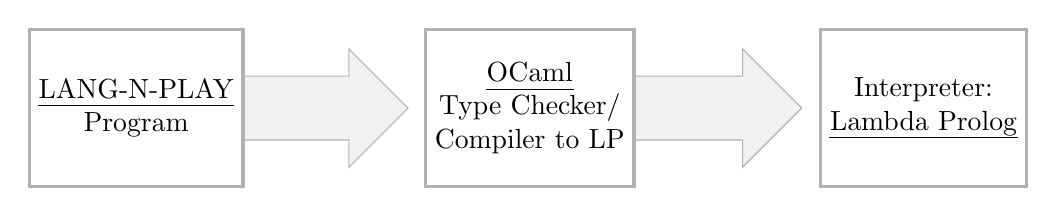
\begin{tikzpicture}[
    squarednode/.style={rectangle, draw=gray!60, fill=white, very thick, minimum size=20mm, align=center},
    thiccboi/.style={single arrow, draw=gray!60, fill=gray!10, minimum width = 15mm, single arrow head extend=3pt, minimum height=25mm}
  ]

  \node[thiccboi] at (2,0) {};
  \node[thiccboi] at (7,0) {};

  \node[squarednode] at ( 0, 0) (fst) {\uline{LANG-N-PLAY}\\Program};
  \node[squarednode] at ( 5, 0) (snd) {\uline{OCaml}\\Type Checker/\\Compiler to LP};
  \node[squarednode] at (10, 0) (trd) {Interpreter:\\\uline{Lambda Prolog}};

  % \draw[arrow] {};


  \end{tikzpicture}
  \caption{Architecture of the LANG-N-PLAY compiler \cite{cimini_effectiveness_2020}.}
  \label{fig:lnp-architecture}
\end{figure}

\subsection{Language Definition}
LANG-N-PLAY provides a domain specific language as means to specify language definitions. It closely resembles how language definitions are usually specified in research \cite{cimini_effectiveness_2020}. The following definition defines a language that has lists and provides an \lstinline{elementAt} operator, which returns the element of a list at a given index.

\begin{lstlisting}
{!
  Type T ::= int | (list T),
  Expression e ::= zero | (succ e) | nil | (cons e e)
                   | (elementAt e e),
  Value v ::= zero | (succ v) | nil | (cons v v),
  Context C ::= (succ E) | (cons C e) | (cons v C)
                | (elementAt C e) | (elementAt v C),
  Environment Gamma ::= [x : T],
  Relation ::= Gamma |- e : T | e --> e,
  StartingCall ::= empty | -e : T | e --> e.

  Gamma |- x : T <== x : T in Gamma,
  Gamma |- zero : int,
  Gamma |- (succ e) : int <== Gamma | - e : int,
  Gamma |- nil : (list T),
  Gamma |- (cons e1 e2) : (list T) <==
           Gamma |- e1 : T /\ Gamma | - e2 : (list T),
  Gamma |- (elementAt e1 e2) : T <==
           Gamma |- e1 : int /\ Gamma | - e2 : (list T),
  (elementAt zero (cons V1 V2)) --> V1,
  (elementAt (succ V) (cons V1 V2)) --> (elementAt V V2)
!}
\end{lstlisting}

In LANG-N-PLAY, the \lstinline|{! ... !}| construct marks a language definition block. Language definitions consist of two parts. A grammar which is defined on lines 2 through 10 and a inference system defined on lines 12 through 21.

It is rather simple to compile language definitions defined in LANG-N-PLAY to $\lambda$Prolog because operational semantics map naturally to logic programming rules \cite{cimini_effectiveness_2020}. The following is a small excerpt of the resulting $\lambda$Prolog code for the given example.

\begin{lstlisting}
typeOf nil (list T).
typeOf (cons E1 E2) (list T) :- typeOf E1 T,
                                typeOf E2 (list T).
typeOf (elementAt E1 E2) T :- typeOf E1 int,
                              typeOf E2 (list T).
step (elementAt zero (cons V1 V2)) V1 :- value V1, 
                                         value V2.
step (elementAt (succ V) (cons V1 V2)) (elementAt V V2)
                                      :- value V1, 
                                         value V2.
\end{lstlisting}

To facilitate developer-defined languages that can be manipulated at runtime, LANG-N-PLAY utilizes an internal representation for languages. This internal representation is of the type:

\begin{lstlisting}
type language (list o) -> expLO.
\end{lstlisting}

The language is represented as a set of its terms. Also, as grammar rules are not required to run a program, LANG-N-PLAY only compiles inference rules.


\subsection{Language Operations}
Currently, LANG-N-PLAY only implements a subset of the features outlined in Section \ref{features-of-language-oriented-programming}. While Cimini intends to implement many of these features in the future \cite{cimini_effectiveness_2020}, for now LANG-N-PLAY only implements the following:

\paragraph{Let-Bindings}
LANG-N-PLAY provides Haskell-style let-bindings. This feature allows for easy reuse of language definitions:

\begin{lstlisting}
let lstLang = {!
  ...
!}
in ...
\end{lstlisting}

The reduction for this functionality is implemented as:

\begin{lstlisting}
  type letLO expLO -> (expLO -> expLO) -> expLO.
  stepLO (letLO V R) (R V) :- valueLO V.
\end{lstlisting}

\paragraph{Language Union}
LANG-N-PLAY also implements the unification of language rules. An extension of the previous example could be realized as follows:

\begin{lstlisting}
let safeLstLang = 
  lstLang U {!
    Expression e ::= oobError,
    Error er ::= oobError
    (elementAt zero nil) --> oobError,
    (ElementAt (succ V) nil) --> oobError,
  !}
\end{lstlisting}

This extension makes sure that an error is raised if a program tries to access an index that is outside the bounds of the list. The resulting $\lambda$Prolog code would be:

\begin{lstlisting}
unionLO
  (language [ ...<lstLang>... ])
  (language [ step (elementAt zero nil) oobError ;
              step (elemntAt (succ V) nil) oobError])
\end{lstlisting}

\paragraph{Rule Removal}
As counterpart to unification LANG-N-PLAY also implements the removal of language rules. To remove one of the rules, added in the previous example, the following is possible:

\begin{lstlisting}
remove (elementAt zero nil) --> oobError
from safeLstLang 
\end{lstlisting}

LANG-N-PLAY compiles this to:

\begin{lstlisting}
  removeLO
    (step (elementAt zero nil) oobError)
    (language [ ...<lstLang>... ;
                step (elementAt zero nil) oobError ;
                step (elemntAt (succ V) nil) oobError])
\end{lstlisting}

Thanks to how equality matching works in $\lambda$Prolog, finding the correct rule to remove, is very lenient. In $\lambda$Prolog \lstinline|(term MyVar)| is equal to \lstinline|(term V)|.

As a drawback, in its current implementation LANG-N-PLAY only allows for the removal of a single rule per operation. Thus, to completely remove the safe list extension from the previous example, four remove-operations would need to be chained.


\subsection{Executing Programs}
To execute programs LANG-N-PLAY provides syntax of the form \lstinline|language > program|. To run a program on the prior example:

\begin{lstlisting}
let lstLang = {! ... !}
in lstlang> elementAt 3 [1, 3, 3, 7]
\end{lstlisting}

This example code would compile to:

\begin{lstlisting}
  execLO (language [ ...<lstLang>... ]) 
         (elementAt 3 [1, 3, 3, 7])
\end{lstlisting}

LANG-N-PLAY can also switch between languages at runtime. Consider a language \lstinline|plusLang| that implements the operation \lstinline|plus|. It would then be possible to use this \lstinline|plusLang| and the previously defined \lstinline|lstLang| interchangeably:

\begin{lstlisting}
  let lstLang = {! ... !}
  in 
  let plusLang = {! ... !}
  in pluslang> plus (lstLang> elementAt 2 [1, 2, 3]) 
                    (lstLang> elementAt 1 [4, 5, 6])
\end{lstlisting}

\section{Related Work}
\label{related-work}

The primary literature for this paper is 'On the Effectiveness of Higher-Order Logic Programming in Language-Oriented Programming.', written by M. Cimini \cite{cimini_effectiveness_2020}. In their work the Author shows how higher-order logic programming is a great fit for implementing language-oriented programming languages. To this end Cimini presents an implementation of LANG-N-PLAY, written in $\lambda$Prolog. LANG-N-PLAY is a language-oriented programming language that was envisioned in \cite{cimini_languages_2018}. To our knowledge, Cimini is currently the only one to investigate the feasibility of implementing language-oriented programming languages using higher-order logic programming.

"Programming with Higher-Order Logic", by Miller and Nadathur is one of the primary knowledge sources for higher-order logic programming. In this work, the authors explain the intricacies of higher-order logic in detail, and show how to use it in $\lambda$Prolog. The two relevant implementations of $\lambda$Prolog are the Teyjus project \cite{noauthor_teyjusteyjus_2022}, as well as ELPI \cite{noauthor_elpi_2022}. Furthermore, the Abella theorem solver \cite{noauthor_abella_nodate} can be used to reason about $\lambda$Prolog programs.

In the past, a number of tools and workbenches were developed to facilitate language-oriented programming. Neverlang \cite{vacchi_neverlang_2015}, Spoofax \cite{kats_spoofax_2010} and Racket \cite{flatt_reference_2010} are among the more noteworthy attempts. All these tools provide a more feature complete and mature environment than LANG-N-PLAY, for developing language-oriented. Nonetheless, LANG-N-PLAY's unique implementation makes it a worthwhile endeavor. In their paper Cimini notes an intention to further improve LANG-N-PLAY in the future and implement features found in other tools, such as language unification and restriction, grammar inheritance, language embedding, and aggregation \cite{cimini_effectiveness_2020}.


\section{Conclusion}

\bibliographystyle{ieeetr}
\bibliography{bibliography}
\end{document}
